\documentclass[a4paper, 11pt]{article}

	\usepackage[algo2e, czech, noline, ruled]{assets/proj3/algorithm2e}
	\usepackage[top=3cm, left=2cm, text={17cm, 24cm}]{geometry}
	\usepackage{graphics, multirow, pdflscape, setspace}
	\usepackage[unicode, hidelinks]{hyperref}
	\usepackage[utf8]{inputenc}
	\usepackage[czech]{babel}
	\usepackage{times}
	
	\urlstyle{same}

\begin{document}

\begin{titlepage}
	\begin{center}
		{\Huge \textsc{Vysoké učení technické v~Brně}\\}
		{\huge \textsc{Fakulta informačních technologií}\\}
		\vspace{\stretch{0.382}}
		{\LARGE Typografie a publikování\,--\,3.\ projekt\\}
		{\Huge Tabulky a obrázky\\}
		\vspace{\stretch{0.618}}
		{\Large \today \hfill Onegen\,Niekto}
	\end{center}
\end{titlepage}

\section{Úvodní strana}

Název práce umístěte do~zlatého řezu a~nezapomeňte uvést \uv{dnešní} (today)
datum a vaše jméno a příjmení.

\section{Tabulky}

Pro sázení tabulek m\r{u}žeme použít buď prostředí\texttt{ tabbing }nebo
prostředí\texttt{ tabular}.

\subsection{Prostředí\texttt{ tabbing}}

Při použití\texttt{ tabbing }vypadá tabulka následovně:
%
\begin{tabbing}
	Vodni melouny \quad  \= \textbf{Cena} \quad \=                \kill
	\textbf{Ovoce}       \> \textbf{Cena}       \> \textbf{Množství} \\
	Jablka               \> 25,90               \> 3\,kg             \\
	Hrušky               \> 27,40               \> 2,5\,kg           \\
	Vodní melouny        \> 35,--               \> 1\,kus            \\
\end{tabbing}

\noindent
Toto prostředí se dá také použít pro sázení algoritm\r{u}, ovšem vhodnější je
použít prostředí\texttt{ algorithm }nebo\texttt{ algorithm2e }(viz sekce
3).

\subsection{Prostředí\texttt{ tabular}}

Další možností, jak vytvořit tabulku, je použít prostředí\texttt{ tabular}.
Tabulky pak budou vypadat takto\footnotemark[1]:

\bigskip
\begin{table}[h!]
	\catcode`\-=12
	\centering
	\begin{tabular}{|l|c|c|}
		\hline
		\multirow{2}{*}{\textbf{Měna}} & \multicolumn{2}{c|}{\textbf{Cena}}                   \\ \cline{2-3}
		                               & \textbf{nákup}                     & \textbf{prodej} \\
		\hline
		EUR                            & 22,705                             & 25,242          \\
		GBP                            & 25,931                             & 28,828          \\
		USD                            & 21,347                             & 23,732          \\
		\hline
	\end{tabular}

	\caption{Tabulka kurz\r{u} k~dnešnímu dni}
	\label{tab:kurz}

\end{table}

\bigskip
\begin{table}[h!]
	\catcode`\-=12
	\centering
	\begin{tabular}{|c|c|}
		\hline
		$A$        & $\neg A$ \\
		\hline
		\textbf{P} & N        \\
		\textbf{O} & O        \\
		\textbf{X} & X        \\
		\textbf{N} & P        \\
		\hline
	\end{tabular}
	%
	\begin{tabular}{|c|c|c|c|c|c|}
		\hline
		\multicolumn{2}{|c|}{\multirow{2}{*}{$A \wedge B$}} & \multicolumn{4}{c|}{$B$}                                            \\\cline{3-6}
		\multicolumn{2}{|c|}{ }                             & \textbf{P}               & \textbf{O} & \textbf{X} & \textbf{N}     \\
		\hline
		\multirow{4}{*}{$A$}
		                                                    & \textbf{P}               & P          & O          & X          & N \\ \cline{2-6}
		                                                    & \textbf{O}               & O          & O          & N          & N \\ \cline{2-6}
		                                                    & \textbf{X}               & X          & N          & X          & N \\ \cline{2-6}
		                                                    & \textbf{N}               & N          & N          & N          & N \\ \cline{2-6}
		\hline
	\end{tabular}
	%
	\begin{tabular}{|c|c|c|c|c|c|}
		\hline
		\multicolumn{2}{|c|}{\multirow{2}{*}{$A \vee B$}} & \multicolumn{4}{c|}{$B$}                                             \\\cline{3-6}
		\multicolumn{2}{|c|}{ }                           & \textbf{P}               & \textbf{O} & \textbf{X} & \textbf{N}      \\
		\hline
		\multirow{4}{*}{$A$}
		                                                  & \textbf{P}               & P          & P          & P          & P  \\ \cline{2-6}
		                                                  & \textbf{O}               & P          & O          & P          & O  \\ \cline{2-6}
		                                                  & \textbf{X}               & P          & P          & X          & X  \\ \cline{2-6}
		                                                  & \textbf{N}               & P          & O          & X          & N  \\ \cline{2-6}
		\hline
	\end{tabular}
	%
	\begin{tabular}{|c|c|c|c|c|c|}
		\hline
		\multicolumn{2}{|c|}{\multirow{2}{*}{$A \rightarrow B$}} & \multicolumn{4}{c|}{$B$}                                             \\\cline{3-6}
		\multicolumn{2}{|c|}{ }                                  & \textbf{P}               & \textbf{O} & \textbf{X} & \textbf{N}      \\
		\hline
		\multirow{4}{*}{$A$}
		                                                         & \textbf{P}               & P          & O          & X          & N  \\ \cline{2-6}
		                                                         & \textbf{O}               & P          & O          & P          & O  \\ \cline{2-6}
		                                                         & \textbf{X}               & P          & P          & X          & X  \\ \cline{2-6}
		                                                         & \textbf{N}               & P          & P          & P          & P  \\ \cline{2-6}
		\hline
	\end{tabular}

	\caption{Protože Kleeneho trojhodnotová logika už je \uv{zastaralá},
		uvádíme si zde příklad čtyřhodnotové logiky}
	\label{tab:log}

\end{table}
\bigskip

\footnotetext[1]{
	Kdyby byl problem s\texttt{ cline,} zkuste se podívat třeba sem:
	\url{http://www.abclinuxu.cz/tex/poradna/show/325037}.
}

\pagebreak

\section{Algoritmy}

Pokud budeme chtít vysázet algoritmus, m\r{u}žeme použít
prostředí\texttt{ algorithm\footnotemark[2] }
nebo\texttt{ algorithm2e\footnotemark[3]}. Příklad použití
prostředí\texttt{ algorithm2e }viz Algoritmus \ref{alg:fslam}.

\bigskip
\begin{algorithm2e}
	\caption{\textsc{FastSLAM}}
	\label{alg:fslam}

	\LinesNumbered
	\setstretch{0.9}
	\SetInd{1em}{1em}
	\SetNlSty{}{}{:}
	\SetNlSkip{-1.2em}
	\SetArgSty{textrm}
	\SetFuncSty{emph}
	\SetAlgoNlRelativeSize{-1}
	\DontPrintSemicolon

	\SetKwFor{For}{for}{do}{end\ for}
	\SetKwFunction{SampleMotion}{sample\_motion\_model}
	\SetKwFunction{MeasureModel}{measurement\_model}
	\SetKwFunction{UpOccupancy}{$updated\_occupancy\_grid$}

	\KwIn{ $(X_{t-1}, u_t, z_t)$}
	\KwOut{ $X_t$}
	\Indentp{1.66em}
	\BlankLine

	$\overline{X_t} = X_t = 0$ \;
	\For{$k = 1$ to $M$}{
	$x_t^{[k]} =$ \SampleMotion{$ u_t, x_{t-1}^{[k]} $} \;
	$\omega_t^{[k]} =$ \MeasureModel{$ z_t, x_t^{[k]}, m_{t-1} $} \;
	$m_t^{[k]} =$ \UpOccupancy{$ z_t, x_t^{[k]}, m_{t-1}^{[k]} $} \;
	$\overline{X_t} = \overline{X_t} \; + $
	$\langle x_x^{[m]} , \omega_t^{[m]} \rangle$ \;
	}
	\For{$k = 1$ to $M$}{
	draw $i$ with probability $\approx \omega_t^{[i]}$ \;
	add $\langle x_x^{[k]} , m_t^{[k]} \rangle$ to $X_t$ \;
	}
	\KwRet{$X_t$}
\end{algorithm2e}

\section{Obrázky}

Do našich článk\r{u} m\r{u}žeme samozřejmě vkládat obrázky. Pokud je obrázkem
fotografie, m\r{u}žeme klidně použít bitmapový soubor. Pokud by to ale mělo
být nějaké schéma nebo něco podobného, je dobrým zvykem takovýto obrázek
vytvořit vektorově.

\begin{figure}[h]
	\centering
	\scalebox{0.4}{
		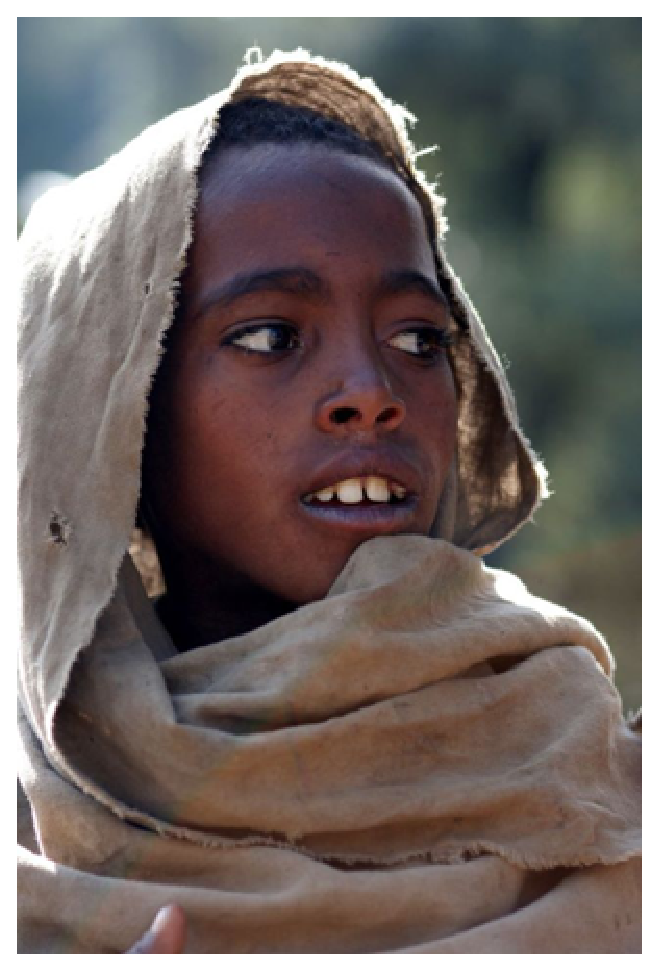
\includegraphics{assets/proj3/etiopan.eps}
		\reflectbox{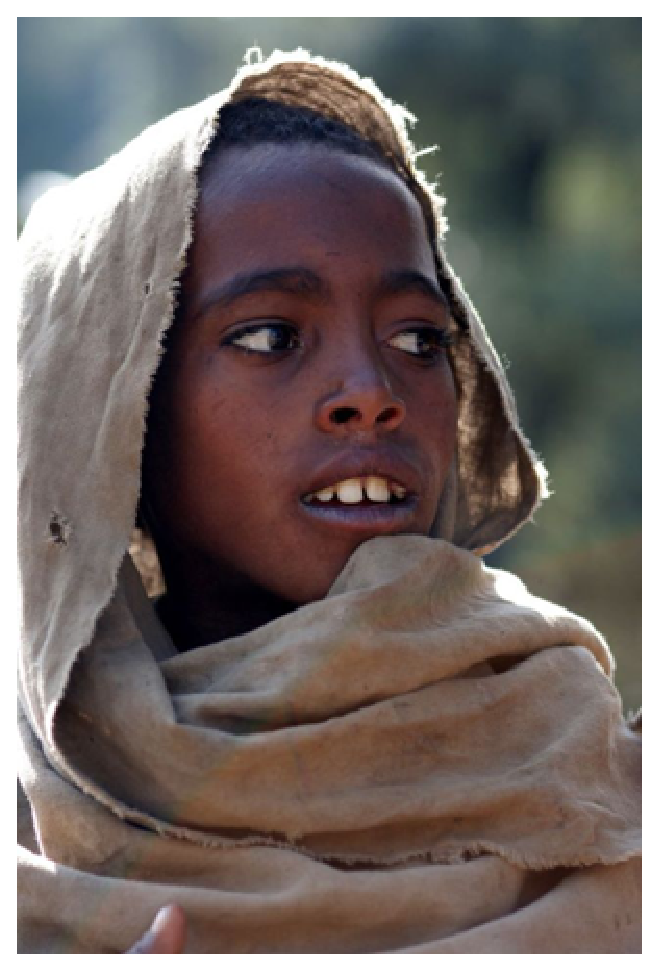
\includegraphics{assets/proj3/etiopan.eps}}
	}

	\caption{Malý Etiopánek a~jeho bratříček}
	\label{fig:etiop}
\end{figure}

\footnotetext[2]{
	Pro nápovědu, jak zacházet s~prostředím\texttt{ algorithm,} m\r{u}žeme
	zkusit tuhle stránku:\\
	\url{http://ftp.cstug.cz/pub/tex/CTAN/macros/latex/contrib/algorithms/algorithms.pdf}.
}

\footnotetext[3]{
	Pro\texttt{ algorithm2e }zase tuhle:
	\url{http://ftp.cstug.cz/pub/tex/CTAN/macros/latex/contrib/algorithm2e/doc/algorithm2e.pdf}.
}

\bigskip
\pagebreak

Rozdíl mezi vektorovým \dots

\begin{figure}[h]
	\centering
	\scalebox{0.4}{
		
\includegraphics{assets/proj3/oniisan.eps}
	}

	\caption{Vektorový obrázek}
	\label{fig:oniisan}
\end{figure}
\bigskip

\noindent
\dots a bitmapovým obrázkem

\begin{figure}[h]
	\centering
	\scalebox{0.6}{
		
\includegraphics{assets/proj3/oniisan2.eps}
	}

	\caption{Bitmapový obrázek}
	\label{fig:oniisan2}
\end{figure}
\bigskip

\noindent
se projeví například při zvětšení.

Odkazy (nejen ty) na obrázky \ref{fig:etiop}, \ref{fig:oniisan} a
\ref{fig:oniisan2}, na tabulky \ref{tab:kurz} a \ref{tab:log} a také
na algoritmus \ref{alg:fslam} jsou udělány pomocí křížových odkazů. Pak je
ovšem potřeba zdrojový soubor přeložit dvakrát.

Vektorové obrázky lze vytvořit i přímo v~\LaTeX{}u, například pomocí
prostředí\texttt{ picture.}
\pagebreak

\end{document}
